% // Esta apresentação -- desenvolvida por Sérgio Mendonça -- está licenciada
% // com uma Licença Creative Commons -- Atribuição (BY) -- Não Comercial (NC)
% // -- Compartilha Igual (SA) 4.0 Internacional. Baseado no trabalho
% // disponível em: https://github.com/sftom/templates/ufrpe/presentation
% //
% // +---------------------------------------------------+
% // | Universidade Federal Rural de Pernambuco          |
% // | Unidade Academica de Garanhuns                    |
% // | Bacharelado em Ciencia da Computacao              |
% // | Sergio Mendonca -- http://bcc.uag.ufrpe.br/~sftom |
% // +---------------------------------------------------+

\documentclass[presentation]{beamer}
\usepackage[utf8]{inputenc}
\usepackage[T1]{fontenc}
\usepackage{graphicx}
\usepackage{longtable}
\usepackage{float}
\usepackage{wrapfig}
\usepackage{soul}
\usepackage{textcomp}
\usepackage{marvosym}
\usepackage{wasysym}
\usepackage{latexsym}
\usepackage{amssymb}
\usepackage{hyperref}
\tolerance=1000
\usepackage[brazil]{babel}

\definecolor{links}{HTML}{2A1B81}
\hypersetup{colorlinks,linkcolor=,urlcolor=links}
\usepackage{lmodern}
\usepackage[utf8]{inputenc} 

\title[Interação Móvel]{Ergonomia e Usabilidade da Interação Móvel}
%\subtitle[]{}
%\author[sergio.mendonca.pro]{\url{http://sergio.mendonca.pro}}
\author[Sérgio Mendonça]{\href{http://bcc.uag.ufrpe.br/\~sftom}{Sérgio Francisco Tavares de Oliveira Mendonça}}
\institute[UFRPE-UAG-BCC]{


\includegraphics[width=6em]{img/logoufrpe.jpg}

\textbf{Universidade Federal Rural de Pernambuco}\\Unidade Acadêmica de Garanhuns\\Bacharelado em Ciência da Computação\\\textbf{Interação Humano-Computador}\\ \url{http://bcc.uag.ufrpe.br/\~sftom}}
%\date{29 de setembro de 2014}

%\usetheme{AnnArbor}\usecolortheme{beaver}
\usetheme{Madrid}\usecolortheme{whale}

\begin{document}
%capa (slide de título)
\begin{frame}[plain]
    \titlepage
\end{frame}

\begin{frame}
\frametitle{Sumário}
\setcounter{tocdepth}{3}
\tableofcontents
\end{frame}
\pgfdeclareimage[height=1.2cm]{logo}{./img/logoufrpe}
\logo{\pgfuseimage{logo}}

\AtBeginSection[]{
\begin{frame}
\frametitle{Agenda}
\tableofcontents[currentsection]
\end{frame}
 }



\section{Experiência móvel e usabilidade} % (fold)
\label{sec:experiencia_movel_e_usabilidade}
\begin{frame}[c]\frametitle{Definindo\ldots}
    \begin{block}{A ``\textbf{experiência do usuário móvel}''?}é definida por Hiltunen (2000) como uma coposição de cinco fatores. Além da \textbf{utilidade} e da \textbf{usabilidade}, o autor acrescentou três outros componentes que, segundo ele, exercem grande influência na opinião geral do usuário sobre o sistema: a \textbf{disponibilidade} do serviço, a \textbf{estética} e todo o \textbf{processo \textit{off-line}}
    \end{block}
\end{frame}


\begin{frame}[c]\frametitle{Componentes da Experiência do Usuário Móvel}
    \begin{figure}[tb]
    	\begin{center}
    		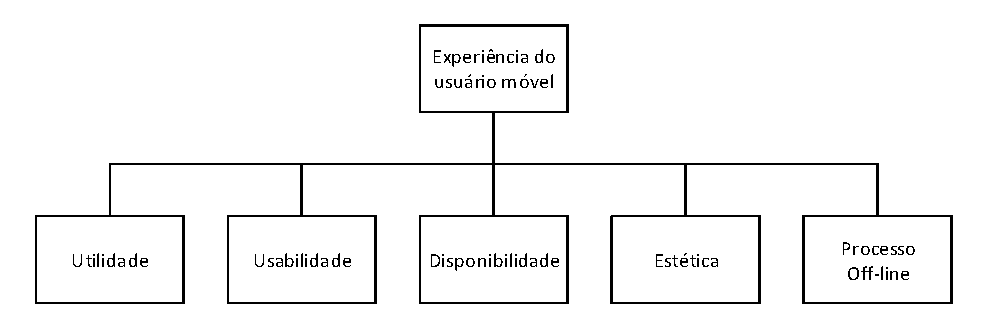
\includegraphics[width=1.0\textwidth]{img/componentes-experiencia-usuario-movel-hiltunen.pdf}
    	\end{center}
    	\caption{Componentes da experiência do usuário móvel. \textit{Fonte: Hiltunen, 2002}}
    	\label{fig:componentes-experiencia-usuario-movel-hiltunen}
    \end{figure}
\end{frame}
% section experiência_móvel_e_usabilidade (end)


\begin{frame}[c]\frametitle{Componentes da experiência do usuário móvel}
    
    \begin{block}{Utilidade}
        refere-se à percepção do usuário móvel em relação ao fato de o serviço lhe agregar algum valor dentro de seu contexto; ou seja, quão vantajosa é a opção de utilizá-lo em relação a outras opções, seja pela localização do usuário, pela disponibilidade de outras opções, pela economia de tempo ou esforço.
    \end{block}

\end{frame}

\begin{frame}[c]\frametitle{Componentes da experiência do usuário móvel}
    
    \begin{block}{Usabilidade}
        é definida como proposto na norma ISO 9241:11, no que diz respeito à eficácia, eficiência e satisfação do usuário na realização de seus objetivos com o sistema interativo.
    \end{block}

\end{frame}

\begin{frame}[c]\frametitle{Componentes da experiência do usuário móvel}
    
    \begin{block}{Disponibilidade do sistema}
        é um fator muito importante para o usuário móvel. O serviço deve estar sempre on-line e funcionando perfeitamente. Longos períodos de espera na transmissão das informações, ausência de sinal, interrupções ou quedas de conexão são extremamente frustrantes. Embora o desenvolvedor não tenha controle sobre a conexão e a área de cobertura das operadoras, ele deve considerar esses fatores no projeto da interação.
    \end{block}

\end{frame}

\begin{frame}[c]\frametitle{Componentes da experiência do usuário móvel}
    
    \begin{block}{Estética}
        refere-se ao apelo visual da aplicação, à sua atratividade para o usuário. As limitações físicas das telas podem restringir as opções do designer em relação à quantidade e à qualidade gráfica da informação que estará disponível. Entretanto, ao contrário dos primeiros computadores de mão, os novos modelos com telas coloridas e de maior resolução já permitem a criação de interfaces mais atraentes.
    \end{block}

\end{frame}

\begin{frame}[c]\frametitle{Componentes da experiência do usuário móvel}
    
    \begin{block}{Processo off-line}
        complementa a experiência do usuário. Assim como para os serviços fornecidos pela web, há diversos elementos que contribuem para a experiência do usuário, mas que não estão relacionados ao projeto da interação, por exemplo, a confiança no nome da empresa que oferece o serviço, a segurança dos dados, além de todo o processo de retaguarda, como o suporte ao usuário ou a rapidez e a qualidade na entrega de uma mercadoria.
    \end{block}

\end{frame}

\begin{frame}[c]\frametitle{Além desses fatores\ldots}
    
    \begin{itemize}
        \item custos de acesso aos serviços de internet móvel;
        \item modelo de cobrança das operadoras.
    \end{itemize}

    \begin{block}{um grande impacto na experiência do usuário\ldots}
        esses fatores exercem grande impacto na experiência do usuário móvel\ldots (principalmente na dificuldade de compreensão dos custos vs. modelo de cobrança). (ROTO, 2006).
    \end{block}
    
\end{frame}


\begin{frame}[c]\frametitle{Outro detalhe\ldots}
    
    é importante destacar também os componentes \textbf{emocionais} da experiência do usuário.

    \begin{block}{Componente \textbf{emocional}}
        não usamos simplesmente um produto, mas nos tornamos \textbf{emocionalmente envolvidos} por ele, e este envolvimento é particularmente intenso quando se trata dos computadores de mão, principalmente os telefones celulares.
    \end{block}

\end{frame}

\section{Contexto da Interação Móvel} % (fold)
\label{sec:contexto_da_interacao_movel}

\begin{frame}[c]\frametitle{Contexto da Interação Móvel: Usuário}
    
    é muito importante entender o usuário móvel e a dinâmica do contexto em que ele está inserido\ldots

    \begin{itemize}
        \item  o \textbf{computador de mesa} é usado para digitar textos, elaborar planilhas eletrônicas, fazer pesquisas na Internet, programar dispositivos e aplicações, ou seja, tarefas que exigem concentração e são executadas durante um longo período de tempo;
        \item já os \textbf{computadores de mão} são voltados para aplicações mais rápidas, executadas em um período de tempo mais curto e extremamente focadas, como verificar o saldo antes de efetuar uma compra, confirmar um voo já reservado, fazer pequenas anotações durante uma reunião.
    \end{itemize}

\end{frame}
% section contexto_da_interação_móvel (end)

\begin{frame}[c]\frametitle{Contexto da Interação Móvel: Fatores a Observar\ldots}

    \begin{block}{O tempo, número reduzido de passos}
    o \textbf{tempo} é um fator muito importante para o usuário móvel, que é mais impaciente e exigente que o usuário do computador de mesa e tende a utilizar serviços que \textbf{permitam a manipulação rápida} da interface e o acesso à informação por meio de \textbf{um número reduzido de passos}. (ERICSSON, 2001).
\end{block}

\end{frame}


\begin{frame}[c]\frametitle{Contexto da Interação Móvel: Fatores a Observar\ldots}

    \begin{block}{Pouco previsível e muito dinâmico\ldots}
    o usuário móvel tem menor capacidade de processar e absorver conteúdo que um usuário que está sentado em frente a um computador de mesa. (RISCHPATER, 2000, p.~33).
    \end{block}
    
    de fato, o usuário de um computador de mão normalmente está envolvido em várias atividades que ocorrem simultaneamente; sua atenção pode estar dividida entre o \textbf{uso do equipamento}, as \textbf{outras atividades} que ele está realizando e o \textbf{ambiente} que o cerca.

\end{frame}

\begin{frame}[c]\frametitle{Aspectos da interação móvel vs. interação fixa}

    \begin{figure}[tb]
        \begin{center}
            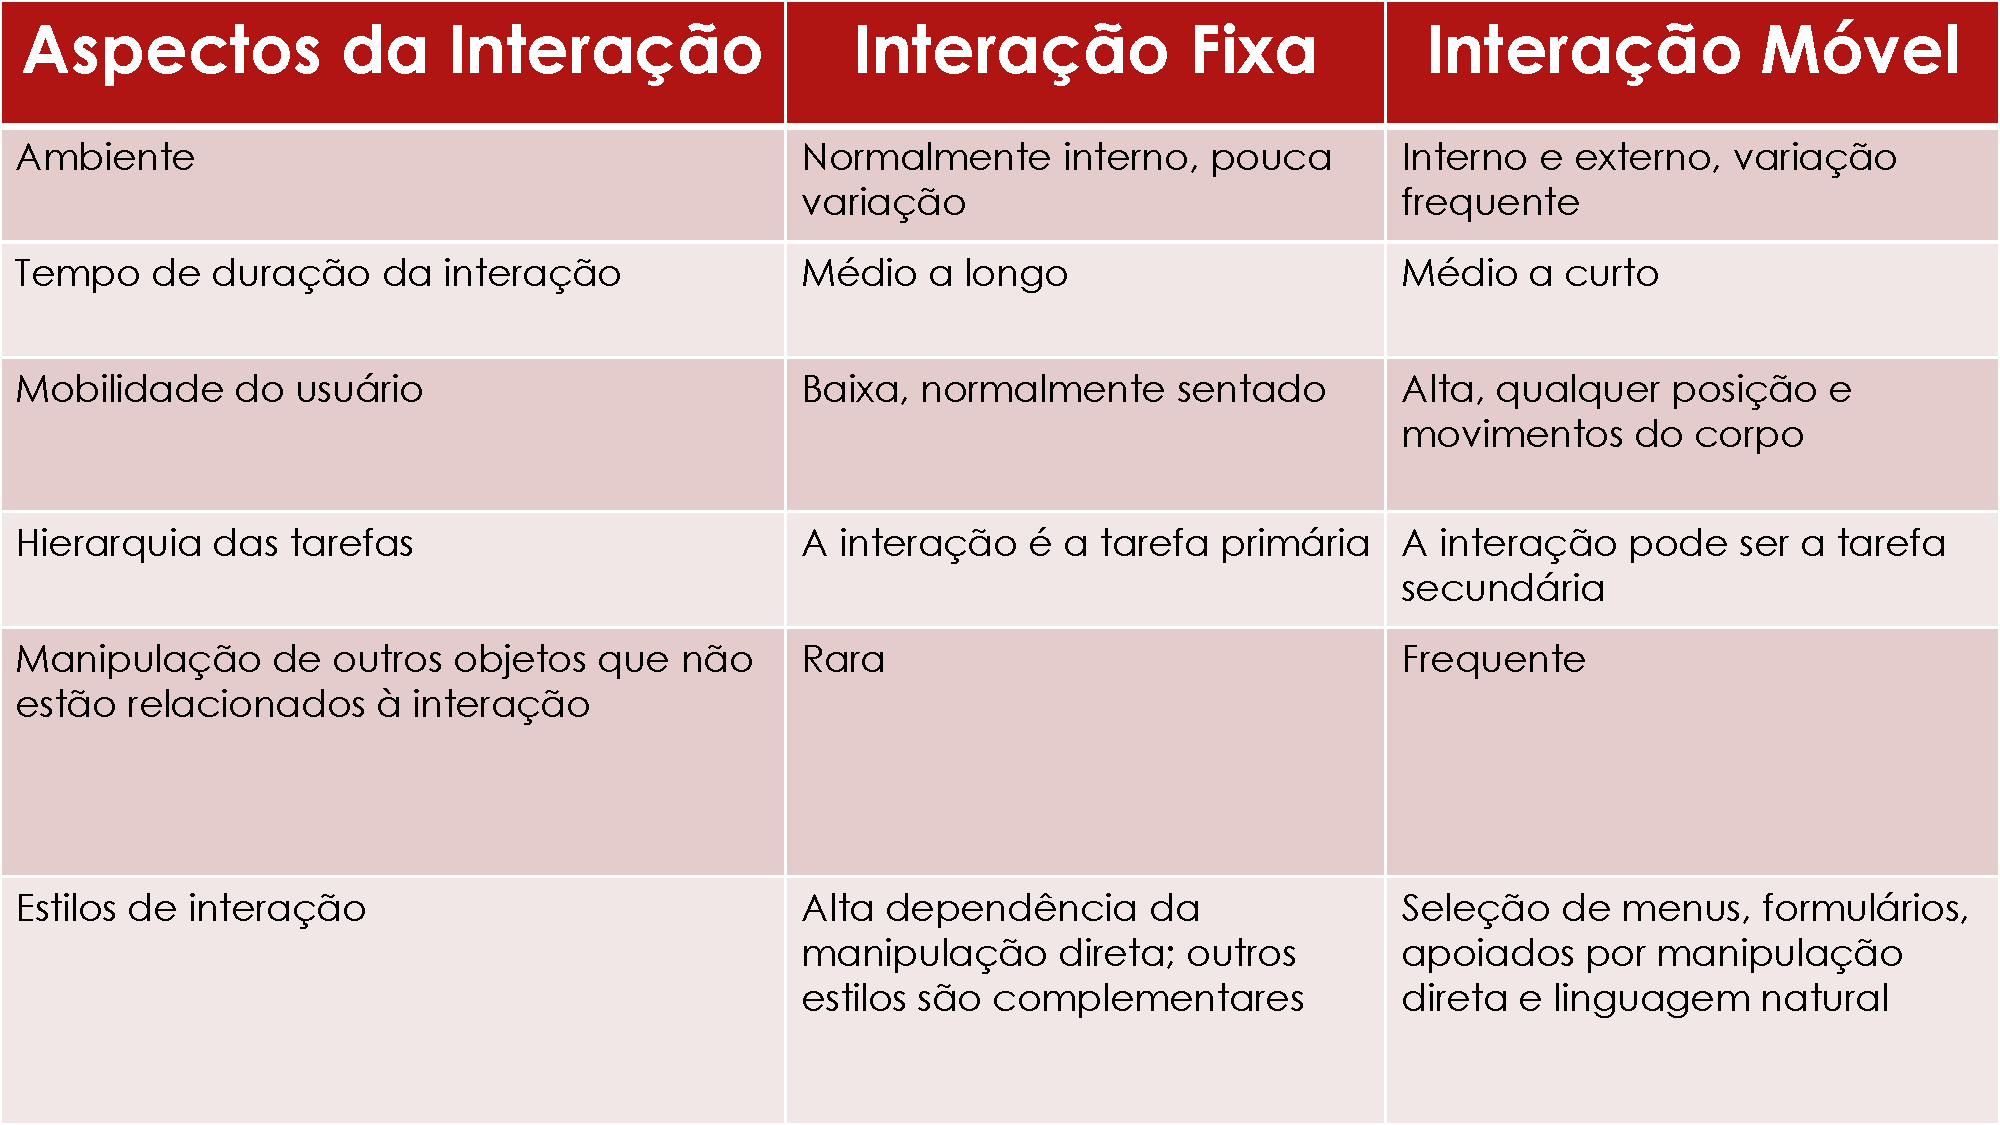
\includegraphics[width=0.95\textwidth]{img/aspectos-interacao-movel-relacao-interacao-fixa.pdf}
        \end{center}
        \caption{Aspectos da interação móvel em relação aos da interação fixa. \textit{Fonte: adapatado de Gorlenko (2003)}}
        \label{fig:aspectos-interacao-movel-relacao-interacao-fixa}
    \end{figure}

\end{frame}

\section{Computadores de Mão} % (fold)
\label{sec:computadores_de_mao}

\begin{frame}[c]\frametitle{O Desafio da nomenclatura}
    
    com o surgimento dessa nova área, foram propostos diversos termos utilizados em inglês:

    \begin{itemize}
        \item mobile devices;
        \item wireless devices;
        \item handheld devices\ldots   
    \end{itemize}

    todos foram traduzidos para o português como:

    \begin{itemize}
        \item computadores portáteis;
        \item computadores sem fio;
        \item computadores de bolso;
        \item micros de mão
        \item dispositivos móveis\ldots
    \end{itemize}

\end{frame}

\begin{frame}[c]\frametitle{Handheld}
    
    \begin{block}{Definição do termo handheld}
        Weiss, em seu livro \textit{Handheld usability} (2002), utilizou o termo \textit{handheld} para designar todo equipamento que atenda às seguintes características:
        \begin{enumerate}[a)]
            \item funcionar sem cabos, exceto temporariamente (recarga, sincronização\ldots);
            \item ser operado facilmente nas mãos, sem necessidade de estar apoiado numa mesa;
            \item permitir a adição de novos aplicativos ou suportar conexão à internet.
        \end{enumerate}
    \end{block}

\end{frame}

\begin{frame}[c]\frametitle{Conceito de Interação Móvel}

    \begin{block}{}
        Gorlenko e Merrick (2003) definem o conceito de interação móvel que se refere à mobilidade, não apenas do equipamento, mas também do usuário.
    \end{block}
 
    alguns autores utilizam o termo FMWC (\textit{Fully Mobile Wirelessly Connected}) para definir equipamentos protáteis que apoiam a interação móvel e que, além disso, possuem conexão sem fio. O usuário ``NÃO'' está mais \textbf{preso} a determinado local: ele pode se movimentar.

    houve uma evolução do computador pessoal em direção à portabilidade, caracterizada por alguns tipos de equipamentos, como observaremos, a seguir.

\end{frame}

\begin{frame}[c]\frametitle{Equipamentos vs. Portabilidade}
    
    \begin{itemize}
        \item \textbf{Desktops}
        \item \textbf{Laptops}
        \item \textbf{Palmtops}
        \item \textbf{Handhelds}
        \item \textbf{Wearables}
    \end{itemize}

    Para ser considerado um computador de mão o equipamento deve:

    \begin{itemize}
        \item \textbf{ser portátil}: facilmente transportado pelo usuário;
        \item \textbf{permitir a mobilidade do usuário}: o usuário deve poder se movimentar livremente durante a interação; 
        \item \textbf{permitir a conexão sem fio}: se for necessário conexão à internet ou a outros equipamentos, para garantir a mobilidade do usuário, o equipamento deve possuir algum tipo de conexão feita pelo ar, sem o uso de fios ou cabos.
    \end{itemize}

\end{frame}

% section computadores_de_mão (end)



\section{Princípios para o Projeto da Interação Móvel} % (fold)
\label{sec:principios_para_o_projeto_da_interacao_movel}

\begin{frame}[c]\frametitle{Princípios para o projeto da interação móvel}
    
    Boa parte das recomendações ergonômicas para o projeto de interface com o usuário de aplicações no desktop se aplica ao projeto das interfaces para os computadores de mão.

    Entretanto, algumas recomendações são específicas para esse contexto, pois consideram as particularidades da interação móvel apresentadas e discutidas a seguir.

    Algumas das principais recomendações para projeto da interface com o usuário para os computadores de mão (WEISS, 2001; CHAN, 2002; GONG, 2004; BALLARD, 2004) são apresentadas a seguir.

\end{frame}

\begin{frame}[allowframebreaks]\frametitle{Projeto de Interface: Recomendações}
    
    \begin{enumerate}
        \item \textbf{Adequação ao contexto do usuário móvel} --- o primeiro passo no projeto de aplicações e serviços para os computadores de mão é analisar se eles são apropriados ao ambiente e às necessidades do usuário móvel. O usuário ``NÃO'' deseja as funções de um computador de mesa: ele quer ter acesso rápido à informação no momento e no local em que mais precisa dela. \newpage
        \item \textbf{Interface não ``miniaturizada''} --- estruturas de navegação, controles e metáforas adequadas a telas grandes, mouse e teclados completos \textbf{podem não ser adequados} à interação móvel. A interface deve ser projetada especialmente para o computador de mão, considerando as limitações físicas do equipamento e a perspectiva do usuário móvel. \newpage
        \item \textbf{Consistência interna e externa} --- além de manter a consistência entre os elementos da interface em diferentes telas de uma mesma aplicação, é importante manter a consistência externa, ou seja, utilizar elementos já conhecidos do usuário presentes na interface da aplicação em outras plataformas. O usuário deve perceber facilmente que se trata da mesma aplicação, independente da plataforma ou do equipamento em que ela é utilizada. Embora os objetos de interação e os estilos de navegação tenham de ser diferentes, alguns aspectos da interface podem ser similares, por exemplo, as cores, a organização das opções nos menus e a terminologia.\newpage
        \item \textbf{Minimização de custo e carga de trabalho} --- o tempo de acesso e o custo dos serviços são fatores críticos para o usuário móvel. Ao utilizar um serviço, acessar um site, por exemplo, o usuário está sendo cobrado por tempo de acesso como em uma ligação de voz, ou por quantidade de informação transmitida, em kbytes. Isto é, independente da tecnologia de seu computador de mão, o usuário vai querer minimizar seus gastos acessando rapidamente a informação, utilizando o menor número de passos possível. Portanto, é importante reduzir o número de cliques e de telas necessárias para executar as tarefas mais frequentes. Nesse sentido, usuários mais experientes devem contar com atalhos que os levem diretamente à informação ou ao serviço desejado. Os ícones, por sua vez, representam soluções de economia não só para a navegação nas telas como também para a carga cognitiva do usuário, pois diminuem a necessidade de memorização, desde haja uma relação natural entre sua representação e seu significado. \newpage 
        \item \textbf{Facilidade de navegação} --- a capacidade limitada das telas, as interrupções frequentes e a possível falta de atenção contribuem para que o usuário móvel se perca com maior frequência na navegação (ele não sabe onde se encontra e qual a relação daquela tela com o restante da aplicação). Assim, é importante definir estruturas de informação e de comandos bastante simples, de modo a que elas sejam compreendidas e lembradas facilmente. Os menus profundos, repletos de submenus, devem dar lugar a menus rasos, mesmo que mais amplos. Toda a aplicação deve apresentar uma página principal, que o usuário terá sempre como ponto de referência. A função \textbf{Voltar à tela anterior} é muito importante para o usuário móvel, devendo estar sempre acessível e visível. Uma função que retorne a outra tela que não a anterior deve ter um nome diferente, como ``Página inicial'', ``Menu principal'' ou outro termo que indique uma localização específica dentro da estrutura de navegação.  \newpage
        \item \textbf{Apoio à seleção de Opções} --- sempre que possível, deve-se fornecer um mecanismo de seleção em vez de solicitar ao usuário que digite a informação. Diante de uma lista de links organizados hierarquicamente, o usuário deve poder diferenciar entre nomes de categorias e os links propriamente ditos. Além disso, ele deve poder diferenciar instantaneamente onde começa e onde termina um link. \newpage
        \item \textbf{Cuidado com a rolagem de tela} --- apesar de alguns equipamentos possuírem teclas que facilitam a rolagem de tela, ela não deve ser utilizada em excesso. À medida que o usuário vai rolando as telas, mais informações precisam ser armazenadas em sua memória de trabalho (capacidade reduzida), pois o que ele não está mais vendo precisa ser lembrado para que a informação possa lhe fazer sentido. Quanto menor a tela, consequentemente menos informação visível, maior a carga cognitiva. Deve-se colocar as informações mais importantes no topo da página, tomando o cuidado de eliminar as linhas em branco. \newpage
        \item \textbf{Apoio às interrupções} --- a interação móvel pode ser interrompida a qualquer momento por eventos externos que distraiam a atenção do usuário, por falhas de conexão da rede ou até mesmo por acabar a bateria do equipamento. A interface deve estar preparada para dar suporte ao usuário quando ele retornar à interação. Para tanto, ela deve minimizar a necessidade de o usuário memorizar informação durante a realização da tarefa, deixando menus sempre visíveis e evitando páginas muito longas. \newpage
        \item \textbf{Apoio à personalização da interface} --- diferentemente dos computadores de mesa, que podem ser compartilhados por vários usuários, os computadores de mão são equipamentos pessoais, na maior parte das vezes usados por uma única pessoa. Telefones celulares e PDAs são carregados para todos os lugares, do escritório ao cinema, como se fossem uma carteira de dinheiro. Além disso, os diversos contextos em que o usuário móvel se encontra podem demandar diferentes necessidades que afetam a usabilidade do sistema.
    \end{enumerate}

\end{frame}


% section princípios_para_o_projeto_da_interação_móvel (end)




\section{Testes de Usabilidade Móvel} % (fold)
\label{sec:testes_de_usabilidade_movel}

\begin{frame}[c]\frametitle{Testes de usabilidade móvel}
    
    \begin{block}{A ergonomia de computadores de mão}
        pode ser avaliada por pessoas mais ou menos especialistas empregando princípios e recomendações já apresentados. Evidentemente, tais pessoas terão o cuidado de analisar e considerar os aspectos do usuário móvel e seu contexto especialmente dinâmico durante suas avaliações.
    \end{block}

\end{frame}

\begin{frame}[c]\frametitle{Testar e medir a usabilidade}
    
    \begin{block}{Testar e medir a usabilidade da interação móvel}
        já a tarefa de testar e medir a usabilidade da interação móvel coloca vários desafios. Os computadores de mão são normalmente utilizados em contextos diversos e extremamente dinâmicos
    \end{block}

\end{frame}

\begin{frame}[c]\frametitle{Testar e medir a usabilidade}
    
    \begin{block}{Questionamentos de técnicas tradionais}
        Muitos pesquisadores (JOHNSON, 1998; PETRIE, 1998; BREWSTER, 2002; WATERSON, 2002) questionam a aplicabilidade das técnicas tradicionais de teste de usabilidade que foram inicialmente desenvolvidas para os computadores de mesa, argumentando que essas técnicas precisam ser revistas e adaptadas à interação móvel.
    \end{block}
\end{frame}

\begin{frame}[c]\frametitle{Testar e medir a usabilidade}
    
    \begin{itemize}
        \item Como reproduzir o contexto do usuário móvel dentro do laboratório?
        \item É possível obter dados confiáveis para a avaliação utilizando um emulador?
        \item É imperativo que os testes sejam realizados em campo, em um contexto próximo do real?
    \end{itemize}

    São várias as pesquisas que procuram encontrar respostas a essas perguntas (KJELDOSKOV, 2003; ZHANG, 2005; HAGEN, 2005)\ldots

\end{frame}

\begin{frame}[c]\frametitle{Testes realizados em laboratório}
    
\begin{itemize}
    \item Os laboratórios são ambientes controlados;
    \item O avaliador pode ter total domínio  sobre a avaliação;
    \item O laboratório de testes é também um ambiente mais confortável para o avaliador;
    \item Local seguro, silencioso e com o qual o avaliador já está acostumado;
    \item Todo o ambiente já está preparado para as avaliações, com todos os equipamentos prontos e conectados.
\end{itemize}

\end{frame}

\begin{frame}[c]\frametitle{Testes realizados em laboratório}
   
    Prós\ldots
    \begin{itemize}
        \item No laboratório podem ser utilizados emuladores (disponibilizados por fabricantes ou desenvolvedores);
        \item Emuladores são indicados quando não se tem acesso ao equipamento real;
        \item Alguns pesquisadores (BOCKER, 1999; KAASINEN, 2000; BUCHANAN, 2001; VYAS, 2002) relatam ser possível obter resultados satisfatórios na avaliação da usabilidade da interface de um computador de mão utilizando um emulador;
    \end{itemize}

\end{frame}
    
\begin{frame}[c]\frametitle{Testes realizados em laboratório}
    Contras
    \begin{itemize}
        \item Os emuladores possuem diversas limitações;
        \item Impossibilidade de avaliar a interação física com o equipamento;
        \item Muitas vezes, a entrada de dados (e interação mesmo) é realizada através de mouse e teclado, certas vezes na tela (caso seja sensível ao toque);
        \item Restrição na seleção da amostra de participantes (necessariamente há a necessidade de ser usuário de computador de mesa);
    \end{itemize}

\end{frame}


\begin{frame}[c]\frametitle{Testes realizados em campo}
    
    \begin{itemize}
        \item Os testes realizados fora do laboratório permitem colocar o usuário em situação mais próxima ao contexto real de uso;
        \item É necessária a utilização de equipamentos como câmeras e microfones móveis e portáteis, que funcionam de forma autônoma;
        \item A realização da avaliação de usabilidade dos computadores de mão em campo não é trivial;
        \item Usuários podem se movimentar à vontade;
        \item Ambiente sujeito à mudanças (barulho ou silêncio; local iluminado ou escuro) etc;
        \item Local desconhecido e imprevisível;
        \item Pessoas podem se aproximar do avaliador ou do entrevistado, o que irá interromper a avaliação.
    \end{itemize}

\end{frame}

\begin{frame}[c]\frametitle{Google Design}
    
\begin{figure}[tb]
    \begin{center}
        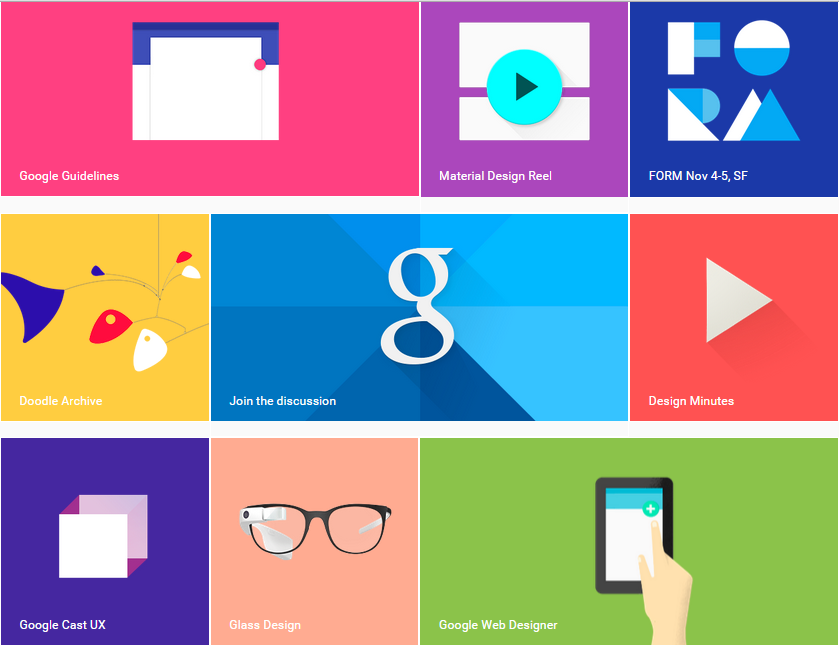
\includegraphics[width=0.7\textwidth]{img/google-com-design.png}
    \end{center}
    \caption{Design Pattern - Google, google.com/design}
    \label{fig:google-com-design}
\end{figure}

\end{frame}

\begin{frame}[c]\frametitle{Android Design}
    
\begin{figure}[tb]
    \begin{center}
        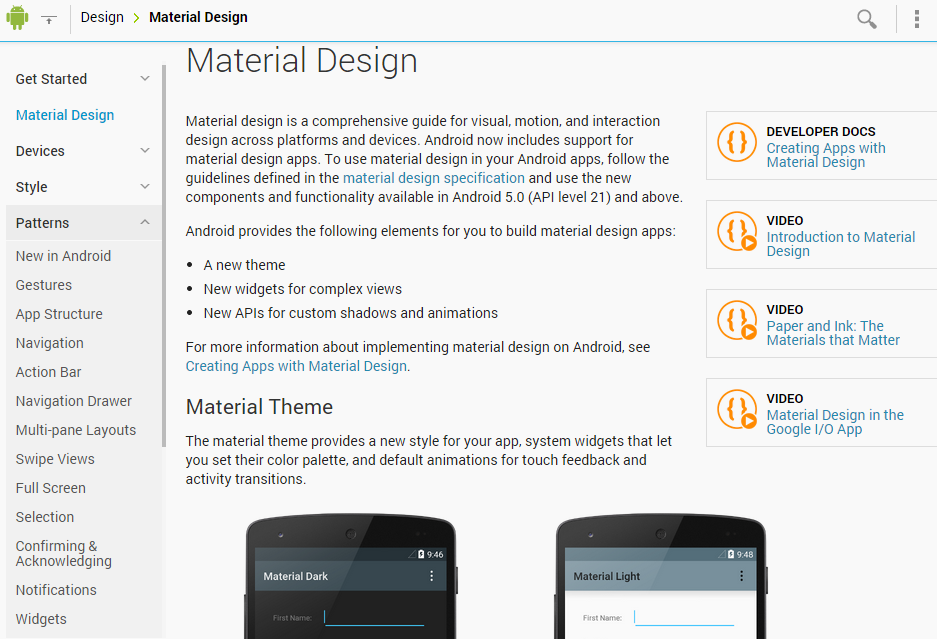
\includegraphics[width=0.8\textwidth]{img/google-android.png}
    \end{center}
    \caption{Design Pattern - Android, developer.android.com/design}
    \label{fig:google-android}
\end{figure}
\end{frame}


\begin{frame}[c]\frametitle{Apple (Mac) Design}
\begin{figure}[tb]
    \begin{center}
        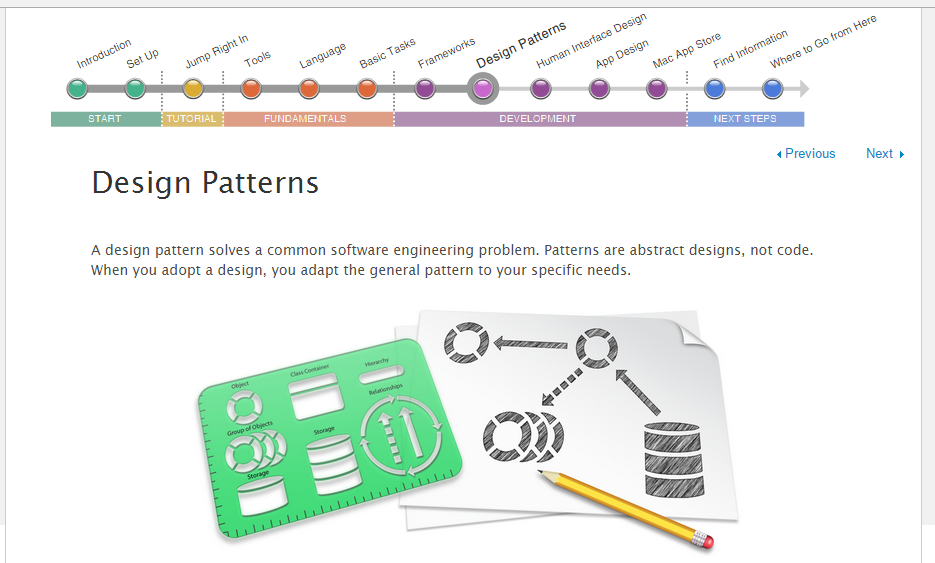
\includegraphics[width=0.8\textwidth]{img/apple-design.png}
    \end{center}
    \caption{Design Pattern - Apple (Mac), developer.apple.com}
    \label{fig:apple-mac}
\end{figure}
\end{frame}

\begin{frame}[c]\frametitle{Apple (iOS) Design}
\begin{figure}[tb]
    \begin{center}
        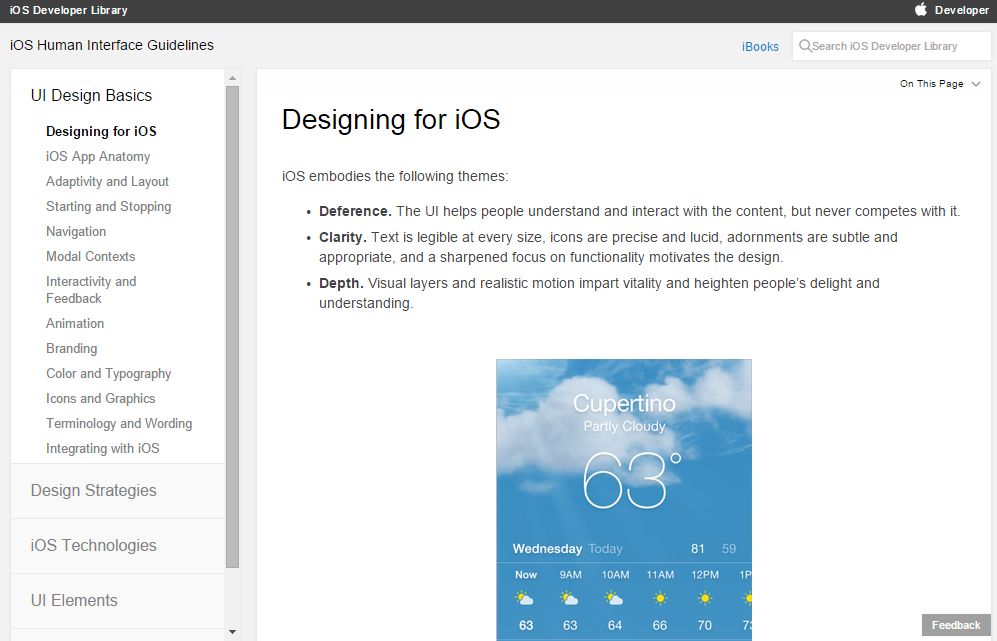
\includegraphics[width=0.8\textwidth]{img/apple-ios-design.png}
    \end{center}
    \caption{Design Pattern - Apple (iOS), developer.apple.com}
    \label{fig:apple-ios}
\end{figure}

\end{frame}

\begin{frame}[c]\frametitle{Microsoft Interation UX}
    
\begin{figure}[tb]
    \begin{center}
        
\includegraphics[width=0.8\textwidth]{img/windows-interation-ux.png}
    \end{center}
    \caption{Design Pattern - Microsoft, dev.windows.com/en-us/design/interaction-ux}
    \label{fig:microsoft-interaction-ux}
\end{figure}
\end{frame}

\section{Sobre o professor}

\begin{frame}
   \frametitle{Sérgio Francisco Tavares de Oliveira Mendonça}
      \begin{columns}
         \begin{column}{0.68\textwidth}
            %% A block
            \begin{enumerate}
            \item Professor
            \begin{itemize}
            \item Linguagem de Programação
            \item Interação Humano-Computador
            \end{itemize}
            \item Interesses
            \begin{itemize}
            \item Web Semântica
            \item Ontologias
            \item Simulações Computacionais
            \end{itemize}
            \item Membro
            \begin{itemize}
            \item \href{http://www.sbc.org.br}{SBC} \href{http://bit.ly/w2zY3N}{(Representante Institucional)}
            \item \href{http://www.acm.org}{ACM}
            \item \href{http://www.ieee.org}{IEEE}
            \item \href{http://www.pmi.org}{PMI}
            \end{itemize}
            \item Para saber mais:
            \begin{itemize}
            \item \href{http://lattes.cnpq.br/6313698968060384}{Currículo CNPq/Lattes}
            \item \href{http://bcc.uag.ufrpe.br/\~sftom}{http://bcc.uag.ufrpe.br/\textasciitilde sftom}
            \end{itemize}
            \end{enumerate}
         \end{column}

         \begin{column}{0.32\textwidth}
            %% A screenshot
            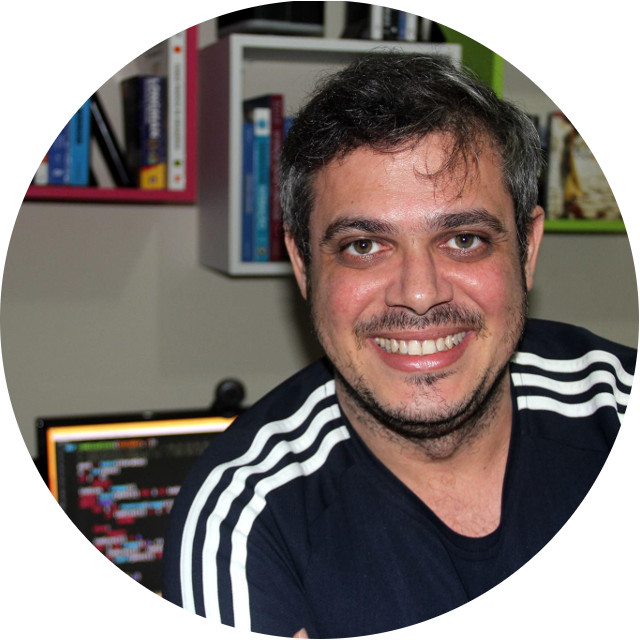
\includegraphics[width=10em]{img/sftom-640x640-circular.jpg}
         \end{column}
      \end{columns}
\end{frame}

 \begin{frame}[c]\frametitle{Creative Commons Licence}
     \begin{figure}[ht]
          \centering
          \caption{\label{fig:by-nc-sa} Creative Commons Licence}
          
\includegraphics[width=0.3\textwidth]{./img/by-nc-sa.jpg}
      \end{figure} 
      Esta apresentação -- desenvolvida por Sérgio Mendonça -- está licenciada com uma Licença Creative Commons -- Atribuição (BY) -- Não Comercial (NC) -- Compartilha Igual (SA) 4.0 Internacional. Baseado no trabalho disponível em:\newline 
      \url{https://github.com/sftom/templates/ufrpe/presentation}
 \end{frame}

\end{document}